% --
% adversarial training

\section{Experiments on Adversarial Pre-Training}\label{sec:exp_adv}
Adversarial pre-training, as already described in detail in \rsec{nn_adv}, is the transfer of learned weights obtained from an adversarial training between a Generator (G) and a Discriminator (D) network from a GAN.
The neural network architecture used for adversarial pre-training is the \texttt{conv-jim} model, as described in \rsec{nn_arch_cnn}.
The \texttt{conv-jim} model initializes its weights from pre-trained weights of its GAN versions, namely the \texttt{adv-d-jim} and \texttt{adv-g-jim}, which are described in \rsec{nn_arch_adv}.
Note that frame-based normalization was applied, which made the training of GANs considerably faster and the weights from G applicable.
Both adversarial pre-training techniques, the adversarial label and dual train, as already explained in \rsec{nn_adv}, were evaluated.

Note that the experiments in this section, like in the previous section, are not meant for comparison to the benchmark networks because of an usage of 500 examples per class instead of the whole dataset.
Also no overfitting mechanism was applied in this experiments.


% --
% label train

\subsection{Impact of Adversarial Label Train}\label{sec:exp_adv_label}
The adversarial label training experiments on the \texttt{conv-jim} architecture with obtained weights from either \texttt{adv-g-jim} or \texttt{adv-d-jim} are presented in \rtab{exp_adv_label_l12}.
\begin{table}[ht!]
\small
\begin{center}
\caption{Experiment with adversarial label pre-training, using either Generator \enquote{g} or Discriminator \enquote{d} weights.}
\begin{tabular}{ M{2cm}  M{2cm}  M{2.5cm}  M{2.5cm} }
\toprule
\textbf{adv iterations} & \textbf{adv model} & \textbf{acc test} & \textbf{acc my} \\
\midrule
100 & g & $75.80 \pm 2.17$ & $85.60 \pm 4.08$ \\
100 & d & $73.57 \pm 1.59$ & $83.20 \pm 6.40$ \\
1000 & g & $74.83 \pm 2.15$ & $85.60 \pm 4.08$ \\
1000 & d & $73.36 \pm 0.86$ & $84.00 \pm 5.06$ \\
\bottomrule
\label{tab:exp_adv_label_l12}
\end{tabular}
\end{center}
\vspace{-4mm}
\end{table}
\FloatBarrier
\noindent
It can be observed that the weights from the Generator network achieves better performances than the weights from the Discriminator network.
\rfig{exp_adv_label_acc_conv-jim} shows in one single accuracy plot the best performing models in the experiments.
\begin{figure}[!ht]
  \centering
  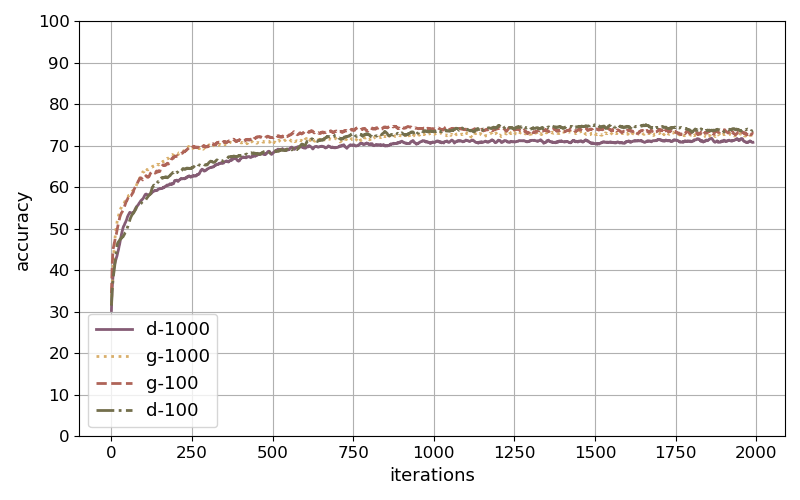
\includegraphics[width=0.48\textwidth]{./5_exp/figs/exp_adv_label_acc_conv-jim.png}
  \caption{Accuracies of the \texttt{conv-jim} model with different adversarial label training and frame-based normalization. The results were smoothed with a 10 epoch average filter.}
  \label{fig:exp_adv_label_acc_conv-jim}
\end{figure}
\FloatBarrier
\noindent
The noise and shift invariance test is shown in \rfig{exp_adv_label_tb_noise_conv-jim} and \rfig{exp_adv_label_tb_shift_conv-jim} respectively.
\begin{figure}[!ht]
  \centering
  \subfigure[D]{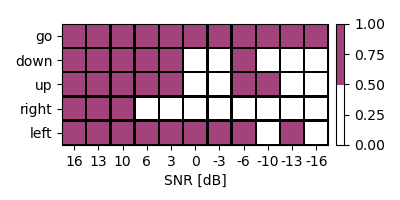
\includegraphics[width=0.35\textwidth]{./5_exp/figs/exp_adv_label_tb_noise_conv-jim_d-100.png}}
  \qquad
  \subfigure[G]{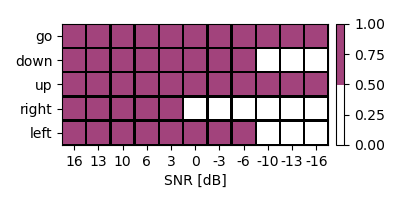
\includegraphics[width=0.35\textwidth]{./5_exp/figs/exp_adv_label_tb_noise_conv-jim_g-100.png}}
  \caption{Noise invariance of the \texttt{conv-jim} model with adversarial label training of 100 epochs and using either the Generator (G) or Discriminator (D) weights.}
  \label{fig:exp_adv_label_tb_noise_conv-jim}
\end{figure}
\FloatBarrier
\noindent
\begin{figure}[!ht]
  \centering
  \subfigure[D]{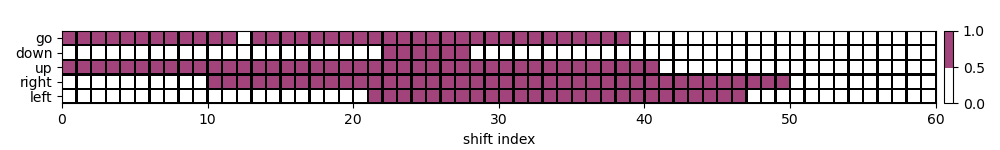
\includegraphics[width=0.48\textwidth]{./5_exp/figs/exp_adv_label_tb_shift_conv-jim_d-100.png}}
  \quad
  \subfigure[G]{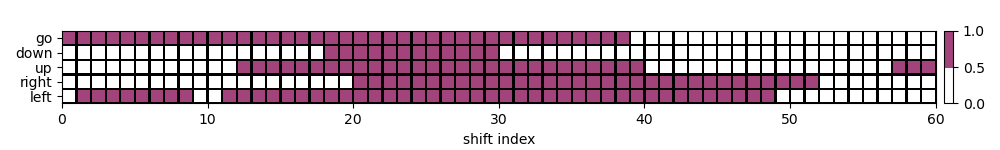
\includegraphics[width=0.48\textwidth]{./5_exp/figs/exp_adv_label_tb_shift_conv-jim_g-100.png}}
  \caption{Shift invariance of the \texttt{conv-jim} model with adversarial label training of 100 epochs and using either the Generator (G) or Discriminator (D) weights.}
  \label{fig:exp_adv_label_tb_shift_conv-jim}
\end{figure}
\FloatBarrier
\noindent
In many experiments the noise and shift invariance show improvements when adversarial pre-training was applied. 


% --
% adv dual train

\subsection{Impact of Adversarial Dual Train}
The adversarial dual training experiments were similar to the adversarial label train ones but without choosing subsets of labels and simply using the same convolutional layer structure for the Generator and Discriminator model like the CNN network.
The experiments are presented in \rtab{exp_adv_dual_l12}.
\begin{table}[ht!]
\small
\begin{center}
\caption{Experiment with adversarial dual pre-training, using either Generator or Discriminator weights.}
\begin{tabular}{ M{2cm}  M{2cm}  M{2.5cm}  M{2.5cm} }
\toprule
\multicolumn{2}{c}{\textbf{Adversarial}} & \multicolumn{2}{c}{\textbf{Accuracy [\%]}}\\
Epochs & Model & Test set & My dataset\\
\midrule
100 & G & $73.53 \pm 1.75$ & $79.20 \pm 7.33$ \\
100 & D & $69.03 \pm 6.53$ & $72.80 \pm 15.88$ \\
1000 & G & $73.53 \pm 1.53$ & $84.00 \pm 4.38$ \\
1000 & D & $72.57 \pm 1.05$ & $83.20 \pm 2.99$ \\
\bottomrule
\label{tab:exp_adv_dual_l12}
\end{tabular}
\end{center}
\vspace{-4mm}
\end{table}
\FloatBarrier
\noindent
The dual experiments achieved worse accuracies for the transfer of Discriminator weights compared to the initializing of the target model with random weights.
The Generator weights however could increase the average accuracy by at least \SI{1}{\percent}.
The dual training is not further evaluated regarding noise and shift invariance because the adv-label-train performed in most cases better.